\documentclass[10pt,xcolor=table]{beamer}

\usetheme[progressbar=frametitle]{metropolis}
\usepackage{appendixnumberbeamer}
\usepackage{hyperref}
\usepackage{tikz}
% \usetikzlibrary{calc,decorations.pathreplacing,snakes}
\usetikzlibrary{calc,decorations.pathreplacing}
\usepackage{multicol}
\usepackage{comment}
\usepackage[portuguese]{babel}
% \usepackage[style=authortitle,backend=bibtex]{biblatex}
\usepackage[style=authortitle,backend=biber]{biblatex}
\addbibresource{references.bib}
\usepackage{subfig}
\usepackage{csquotes}
\usepackage{caption}
% \usepackage{tikz}
% \usetikzlibrary{arrows.meta,positioning}

\hypersetup{colorlinks=true,linkcolor=,urlcolor=blue}

\expandafter\def\expandafter\insertshorttitle\expandafter{%
  \insertshorttitle\hfill%
  \insertframenumber\,/\,\inserttotalframenumber}

\newcommand{\hideFromPandoc}[1]{#1}
\hideFromPandoc{
  \let\Begin\begin
  \let\End\end
}

\newcommand{\verbatimfont}[1]{\renewcommand{\verbatim@font}{\ttfamily#1}}

\newcommand{\PR}[1]{\ensuremath{\left[#1\right]}}
\newcommand{\PC}[1]{\ensuremath{\left(#1\right)}}
\newcommand{\chav}[1]{\ensuremath{\left\{#1\right\}}}

\usepackage{booktabs}
\usepackage[scale=2]{ccicons}

\usepackage{pgfpages} % for multiple-screen presentations
% \setbeameroption{show notes on second screen}
% \setbeameroption{show notes on second screen=right} % Both

\usepackage{pgfplots}
\usepgfplotslibrary{dateplot}

\usepackage{xspace}
\newcommand{\themename}{\textbf{\textsc{metropolis}}\xspace}


\setbeamertemplate{frame footer}{
\includegraphics[height=0.5cm]{figs/logos.png}}

\setbeamercolor{background canvas}{bg=white}

% \setbeamertemplate{sections/subsections in toc}[ball]
\setbeamertemplate{section in toc}[sections numbered]
\setbeamertemplate{subsection in toc}[ball unnumbered]
\setbeamerfont{footnote}{size=\tiny}

\setbeamertemplate{blocks}[rounded][shadow]

\renewcommand{\footnotesize}{\tiny}
\renewcommand*{\bibfont}{\tiny}

\makeatletter
\renewcommand\@makefntext[1]{%
  \noindent
  \hangindent=5em   % recuo aplicado em TODAS as linhas
  \hangafter=0      % aplica após a primeira linha
  \makebox[1em][r]{\@thefnmark.\,}#1}
\makeatother

% Main slide
\title{Da Evolução das Redes Móveis \\ao Open RAN}
% \subtitle{Subtitle}
\date{\today}
% \date{October 31, 2024}
\author{\textbf{Prof. Dr. Paulo Ditarso Maciel Jr. (\href{mailto:paulo.maciel@ifpb.edu.br}{paulo.maciel@ifpb.edu.br})}}
\institute{
\centering
\normalsize
\vspace{0.5cm}
{\Large \textbf{Desagregação, Virtualização e Novos Paradigmas em Telecom}}\\
\vspace{0.5cm}
{\small \textbf{Aula modelo para a\\ \href{https://www.cesar.school/especializacao/open-ran/}{\textit{Especialização em Open RAN: Redes Abertas e Tecnologias Emergentes}}.}} \\
\vspace{0.5cm}
{\scriptsize
\texttt{\$ git clone \href{https://github.com/pdmjr/network_openran.git}{https://github.com/pdmjr/network\_openran.git}}
}
}

\titlegraphic{\hfill
\includegraphics[height=1.1cm]{figs/logos.png}}

\begin{document}

\maketitle

% Slides iniciais

\begin{frame}
    \frametitle{Disclaimer\footnote{Todas as figuras utilizadas nesta apresentação estão publicamente disponíveis em sites, artigos científicos ou são licenciadas sob a \textit{Creative Commons}.}}
    \begin{itemize}
        \item Esta apresentação tem caráter introdutório e não busca esgotar os temas aqui abordados.
        \item Para um estudo mais aprofundado, é imprescindível a leitura dos livros e materiais indicados.
    \end{itemize}
    \begin{figure}
        \centering
        \includegraphics[width=0.6\textwidth]{figs/questionmark.jpg}
    \end{figure}
    \vspace{0.8cm}
\end{frame}

\begin{frame}{Objetivos da Aula}
\begin{itemize}
  \item Compreender a evolução das redes móveis até o 5G
  \item Discutir desagregação e virtualização de funções de rede
  \item Introduzir o conceito de Open RAN e seus impactos
  \item Analisar oportunidades e desafios
\end{itemize}
\end{frame}

% Slide de Agenda
\begin{frame}
    \frametitle{Agenda}
    \tableofcontents
\end{frame}

% Parte 1: Introdução
\section{Introdução à Evolução}

\begin{frame}{Linha do Tempo das Redes Móveis}
\begin{columns}
    \begin{column}{0.45\textwidth}
        \begin{itemize}
            \item 1G: Voz analógica
            \item 2G: Digital, SMS
            \item 3G: Dados móveis iniciais
            \item 4G: LTE, banda larga IP
            \item 5G: eMBB, mMTC, URLLC
        \end{itemize}        
    \end{column}
    \begin{column}{0.55\textwidth}
        \vspace{1cm}
        \begin{figure}
            \centering
            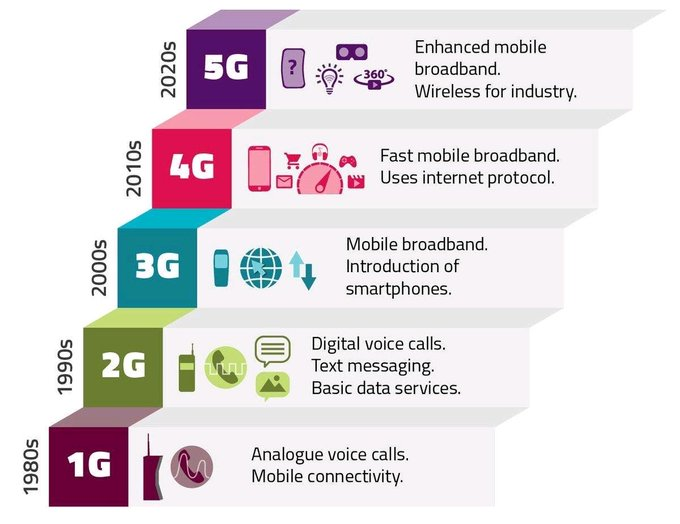
\includegraphics[width=\linewidth]{figs/Network-Generation-Progression.jpg}
            \caption{Telefonia móvel\footnote{\href{https://galooli.com/glossary/what-is-a-network-generation/}{https://galooli.com/glossary/what-is-a-network-generation/}}}
            \label{fig:placeholder}
        \end{figure}
    \end{column}
\end{columns}

\end{frame}

\begin{frame}{Tendências Tecnológicas}
\begin{itemize}
  \item Mais banda e menor latência
  \begin{itemize}
    \item \textbf{Largura de banda ampliada}: suporte a taxas de dezenas de Gbps com novas faixas de espectro, incluindo ondas milimétricas.  
    \item \textbf{Redução da latência}: níveis próximos de 1 ms, viabilizando aplicações em tempo real.  
    \item \textbf{Impacto prático}: telemedicina (cirurgias remotas), realidade virtual imersiva, controle de sistemas industriais críticos.  
  \end{itemize}
  \item Maior densidade de dispositivos
  \begin{itemize}
    \item \textbf{Crescimento exponencial}: milhões de dispositivos conectados% (/km²).  
    \item \textbf{Soluções tecnológicas}: massive MIMO, beamforming e uso de small cells.  
    \item \textbf{Cenários típicos}: centros urbanos, estádios, fábricas inteligentes e ambientes de alta concentração populacional.  
    \item \textbf{Desafio}: garantir eficiência energética e escalabilidade sem perda de qualidade de serviço.  
  \end{itemize}
  % \item Casos de uso: IoT, RA, veículos conectados
\end{itemize}
\end{frame}

\begin{frame}{Casos de uso emergentes}
\begin{itemize}
  \item \textbf{IoT (Internet das Coisas)}: suporte a bilhões de sensores e atuadores, baixo consumo de energia, comunicações massivas e esporádicas.  
  \item \textbf{Realidade Aumentada (RA)}: necessidade de sincronização imediata entre mundo físico e digital, alta taxa de transmissão e baixíssima latência.  
  \item \textbf{Veículos conectados (V2X)}: comunicações ultraconfiáveis para navegação segura, prevenção de acidentes e coordenação entre veículos autônomos.  
  \item \textbf{Visão futura}: redes adaptáveis e programáveis que suportem simultaneamente diferentes requisitos de QoS.  
\end{itemize}
\end{frame}

\begin{frame}
    \frametitle{Arquitetura do 5G}
    \begin{itemize}
        \item \textbf{Rede de Acesso por Rádio (RAN)}: Nova radiofrequência e técnicas avançadas de transmissão.
        \item \textbf{Rede Central (Core)}: Baseada em software, mais flexível e ágil.
        \item \textbf{Suporte Multisserviço}: \textit{Network slicing} para diferentes tipos de serviços.
    \end{itemize}
    \begin{figure}
        \centering
        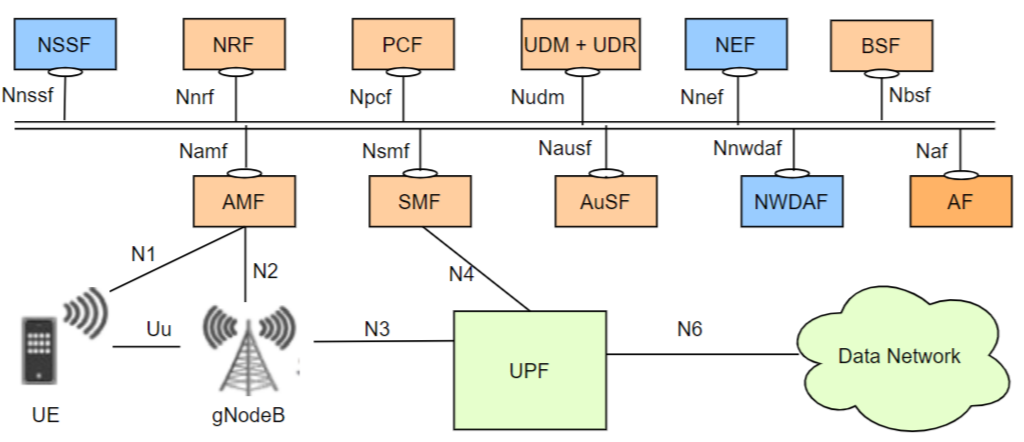
\includegraphics[width=0.7\textwidth]{figs/ArquiteturaGeral5G}
        \caption{Arquitetura Geral do 5G\footcite{5G_architecture}}
    \end{figure}
    \vspace{0.4cm}
\end{frame}

\begin{frame}
    \frametitle{Características Técnicas do 5G}
    \begin{itemize}
        \item \textbf{Velocidade}: Até 20 Gbps.
        \item \textbf{Latência}: Menos de 1 ms.
        \item \textbf{Conectividade Massiva}: Suporte para até 1 milhão de dispositivos por km².
        \item \textbf{Eficiência Espectral}: Utilização otimizada do espectro.
    \end{itemize}
    \begin{figure}
        \centering
        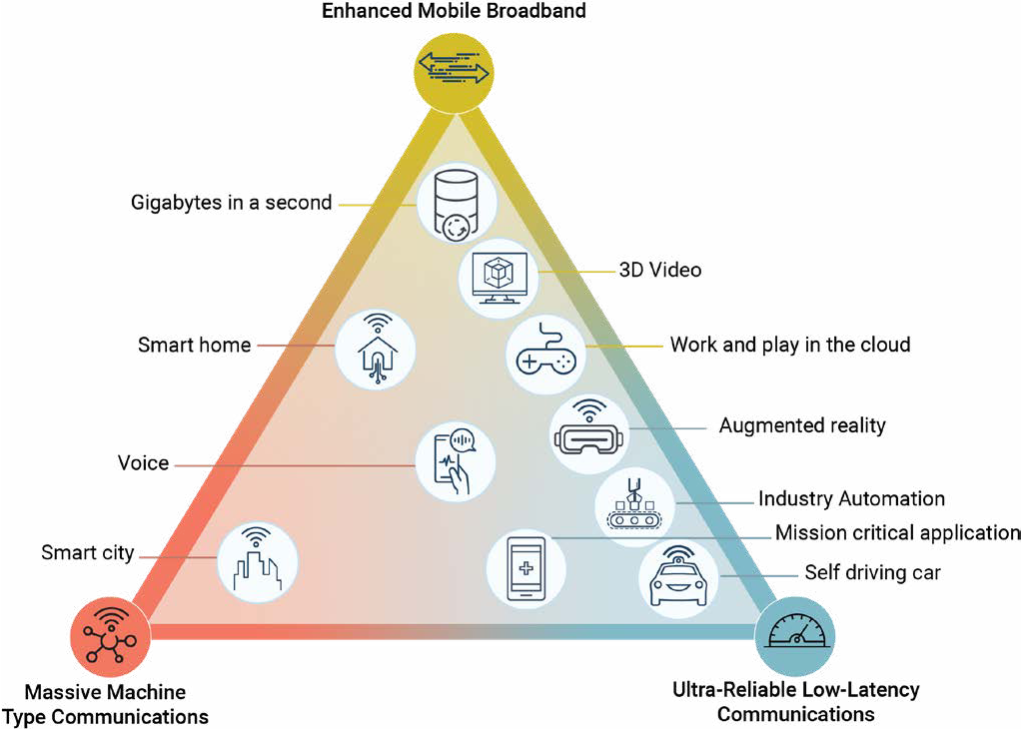
\includegraphics[width=0.5\linewidth]{figs/5G_verticais.png}
        \caption{Requisitos para diferentes tipos de aplicações\footnote{\href{https://www.cio.gov/assets/files/Framework-to-Conduct-5G-Testing-508.pdf}{https://www.cio.gov/assets/files/Framework-to-Conduct-5G-Testing-508.pdf}}}
    \end{figure}
\end{frame}

% Parte 2: Desagregação e Virtualização
\section{Desagregação e Virtualização}

\begin{frame}{Redes Tradicionais vs Virtualizadas}
\begin{itemize}
  \item \textbf{Antes:} nas redes legadas, o hardware (roteadores, switches, firewalls) era projetado de forma proprietária, com software integrado e fechado.  
  \item \textbf{Agora:} as funções de rede foram desacopladas e podem rodar em servidores COTS (\textit{Commercial Off-The-Shelf}), equipamentos comuns de TI, o que reduz custos e aumenta a flexibilidade.  
  \item \textbf{Exemplo ilustrativo:} antes era como comprar um aparelho “tudo em um”; agora é possível usar peças modulares conectadas, escolhendo cada componente de acordo com a necessidade.  
\end{itemize}
\end{frame}

\begin{frame}{Tecnologias Habilitadoras}
\begin{itemize}
  \item \textbf{NFV (\textit{Network Functions Virtualization}):} permite que funções como firewall, load balancer ou EPC (núcleo de rede 4G/5G) sejam executadas em máquinas virtuais ou containers.  
  \item \textbf{SDN (\textit{Software Defined Networking}):} separa o plano de controle (decisões sobre como rotear pacotes) do plano de dados (encaminhamento físico).  
  \item \textbf{Benefícios combinados:} mais automação, facilidade de escalar serviços e redução de CAPEX/OPEX.  
  \item \textbf{Analogia:} NFV é como instalar diferentes aplicativos em um mesmo computador, e SDN é como ter um “sistema operacional central” que coordena todos eles.  
\end{itemize}
\end{frame}

\begin{frame}
    \frametitle{Virtualização das Funções de Rede (NFV)}
    \begin{itemize}
        \item \textbf{Definição}: Abstração das funções de rede do hardware proprietário, executando-as em ambiente virtualizado.
        \item \textbf{Componentes Principais}: VNF (Funções de Rede Virtualizadas), NFVI (Infraestrutura de Virtualização).
        \item \textbf{Vantagens}: Redução de custos, flexibilidade, rapidez na introdução de serviços.
    \end{itemize}
\end{frame}

\begin{frame}
    \frametitle{Arquitetura NFV}
    \begin{itemize}
        \item \textbf{Virtualização do EPC (\textit{Evolved Packet Core})}: Gestão centralizada e flexível do core da rede.
        \item \textbf{vRAN (\textit{Virtualized Radio Access Network})}: Otimização da rede de acesso rádio.
        \item \textbf{\textit{Edge Computing}}: Suporte a aplicações de baixa latência e alta demanda.
    \end{itemize}
    \begin{figure}
        \centering
        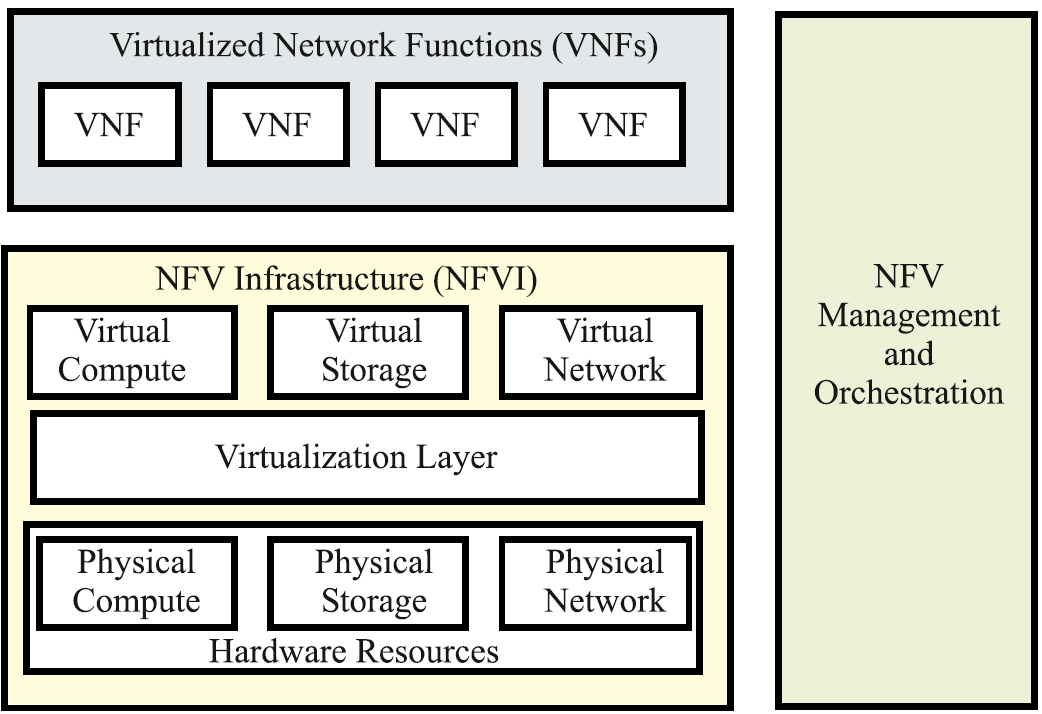
\includegraphics[width=0.45\linewidth]{figs/ArquiteturaNFV.png}
        \caption{Arquitetura geral NFV\footcite{NFV_architecture}}
    \end{figure}
\end{frame}

\begin{frame}{Redes Definidas por Software (SDN)}
    \begin{itemize}
        \item \textbf{Definição}: Arquitetura de rede que separa o plano de controle do plano de dados.
        \item \textbf{Componentes Principais}: Aplicações de rede, controlador SDN, switches programáveis, interfaces.
        \item \textbf{Vantagens}: Flexibilidade, centralização do controle, automação.
    \end{itemize}
    \begin{figure}
        \centering
        \subfloat[Tradicional]{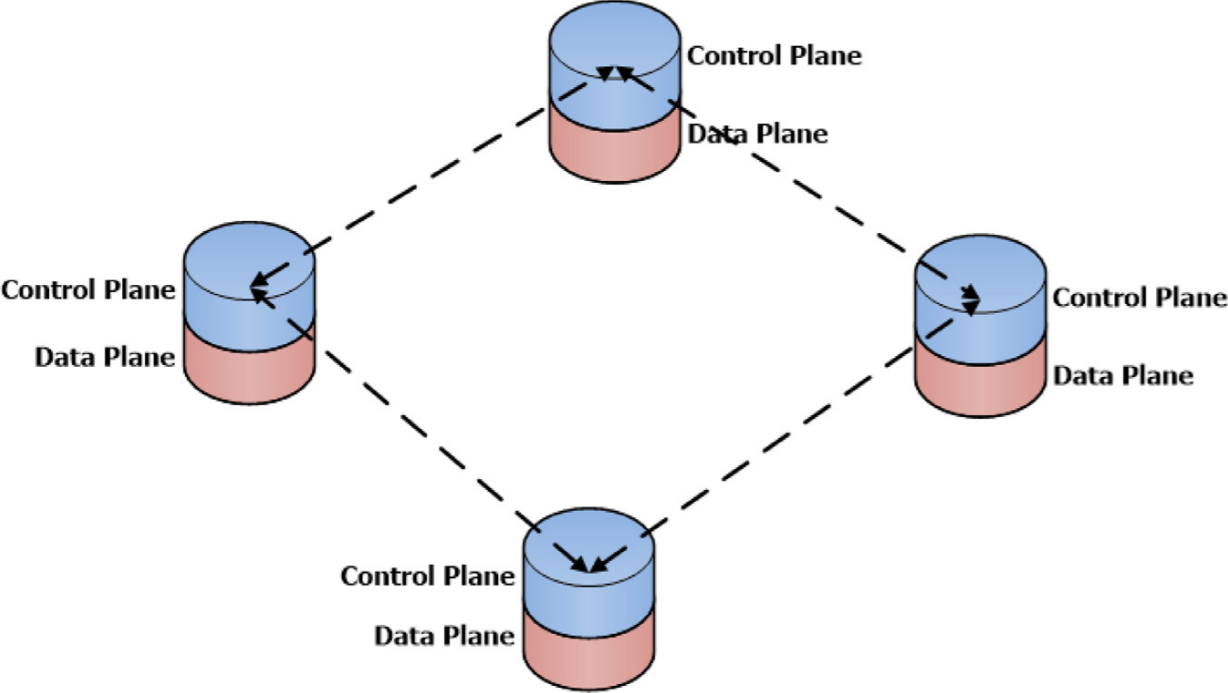
\includegraphics[width=0.45\linewidth]{figs/rede_tradicional.png}}\qquad
        \subfloat[SDN]{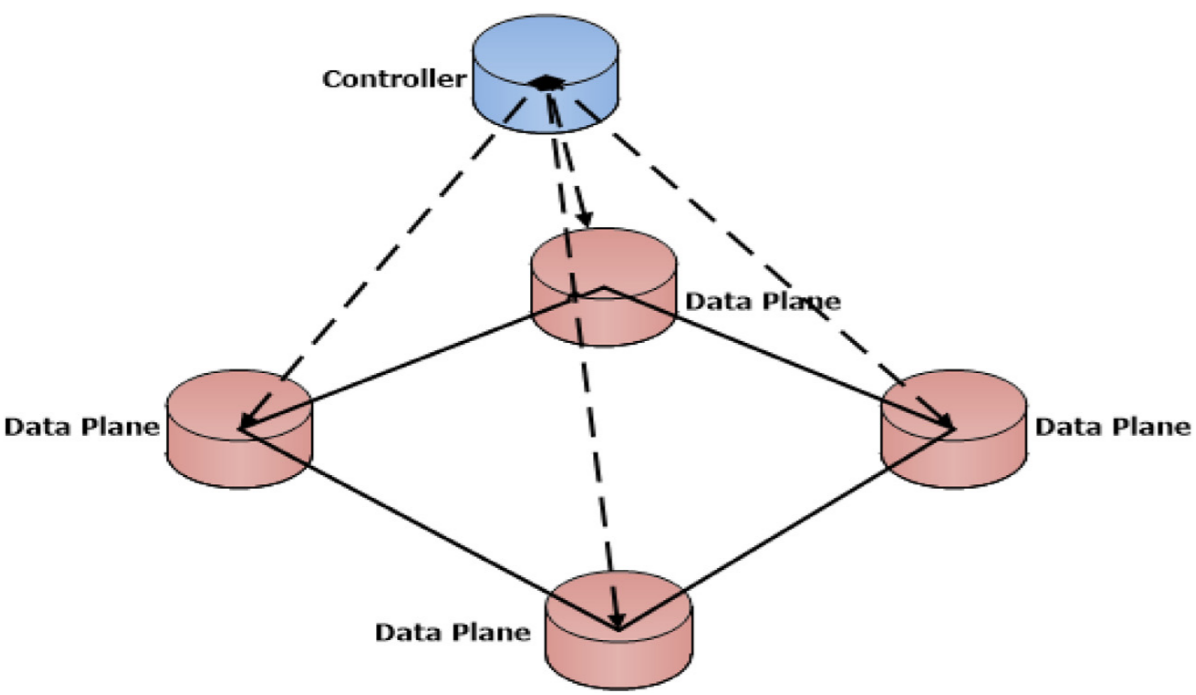
\includegraphics[width=0.45\linewidth]{figs/rede_sdn.png}}
        \caption{Redes tradicionais vs SDN\footcite{Plane_Separation}}
        \end{figure}
\end{frame}

\begin{frame}{Arquitetura SDN}
    \begin{columns}
        \begin{column}{0.55\textwidth}
            \begin{itemize}
                \item \textbf{Plano de Aplicação}: Controle dos recursos via programação.
                \item \textbf{Plano de Controle}: Gerência centralizada dos recursos de rede.
                \item \textbf{Plano de Dados}: Dispositivos de comutação físicos ou virtuais.
                \item \textbf{Interfaces}: Comunicação entre os planos, ao norte (REST), sul (OpenFlow, P4), leste, oeste (API dos controladores).
        \end{itemize}            
        \end{column}
        \begin{column}{0.45\textwidth}
            \vspace{1cm}
            \begin{figure}[h]
                \centering
                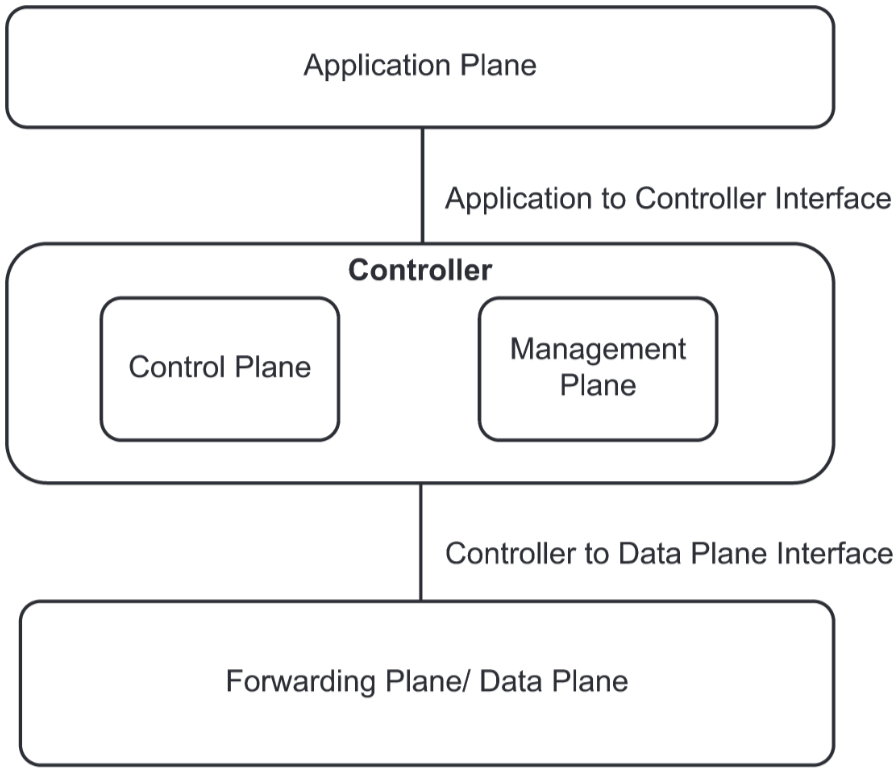
\includegraphics[width=\textwidth]{figs/SDN_arquitetura.png}
                \caption{Arquitetura SDN\footcite{Recommended_SDN_Wireless}}
            \end{figure}
        \end{column}
    \end{columns}
\end{frame}

\begin{frame}{Fatiamento de Rede (\textit{Network Slicing})}
    \begin{itemize}
        \item \textbf{Definição}: Técnica que permite a criação de múltiplas redes virtuais independentes sobre uma única infraestrutura física, otimizadas para atender diferentes requisitos de serviços e aplicações dentro de uma rede 5G.
        \item \textbf{Componentes Principais}: NFV e SDN.
        \item \textbf{Vantagens}: Garantir QoS, agilidade de implantação, personalizar e otimizar recursos de rede para diferentes serviços.
    \end{itemize}
\end{frame}

\begin{frame}{Integração com Operadores de Telecom}
    \begin{figure}[h]
        \centering
        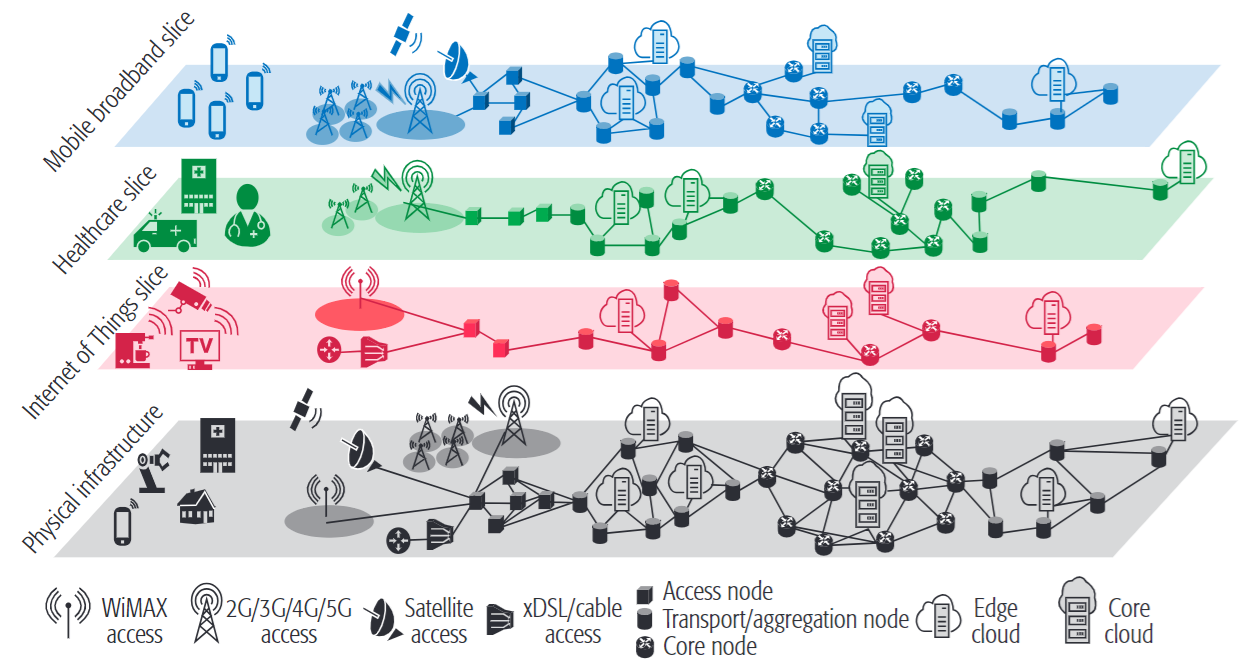
\includegraphics[width=\textwidth]{figs/Network_Slicing.png}
        \caption{Fatiamento de redes\footcite{Network_Slicing}}
    \end{figure}
\end{frame}

\begin{frame}{Desagregação em Telecom}
\begin{itemize}
  \item \textbf{Separação de funções:} no 5G, a RAN (Rede de Acesso Rádio) é dividida em RU (unidade de rádio), DU (unidade distribuída) e CU (unidade centralizada).  
  \item \textbf{Interfaces abertas:} definidas por padrões (ex.: eCPRI, F1, E2), permitem interoperabilidade entre equipamentos de diferentes fornecedores.  
  \item \textbf{Impacto:} facilita a entrada de novos \textit{players} e aumenta a competitividade no mercado.  
  \item \textbf{Exemplo:} uma operadora pode usar a RU da Nokia, a DU da Intel e a CU da Ericsson, todos integrados por interfaces abertas.  
\end{itemize}
\end{frame}

\begin{frame}{Benefícios da Desagregação}
\small
\begin{itemize}
  \item \textbf{Separação hardware/software} $\rightarrow$ menor dependência de fornecedores proprietários.
  \item \textbf{Arquitetura modular (RU, DU, CU)} $\rightarrow$ flexibilidade na evolução e no dimensionamento da rede.
  \item \textbf{Interfaces abertas/padronizadas} (3GPP, O-RAN, ETSI) $\rightarrow$ interoperabilidade real.
  \item \textbf{Ambiente multifornecedor} $\rightarrow$ redução de custos e aumento da concorrência.
  \item \textbf{Escalabilidade seletiva} $\rightarrow$ expande apenas o módulo necessário (otimiza CAPEX/OPEX).
  \item \textbf{Automação e programabilidade} (SDN, APIs) $\rightarrow$ gestão centralizada e operações mais inteligentes.
  \item \textbf{Inovação acelerada} $\rightarrow$ entrada de novos \textit{players} e serviços lançados mais rapidamente.
\end{itemize}
\end{frame}


% Parte 3: Open RAN

\section{O Conceito de Open RAN}

\begin{frame}{Diferenças: Open RAN, O-RAN e OpenRAN}
% \small
\begin{itemize}
  \item \textbf{Open RAN (conceito genérico)}  
    \begin{itemize}
      \item Termo amplo que se refere à \textbf{abertura e desagregação} das redes de acesso de rádio (RAN).  
      \item Não está ligado a um grupo ou organização específica.  
      \item Objetivo: evitar o \textit{vendor lock-in} e permitir múltiplos fornecedores.
    \end{itemize}

  \item \textbf{O-RAN (O-RAN Alliance)}  
    \begin{itemize}
      \item Iniciativa formal liderada por operadoras globais (ex.: AT\&T, China Mobile, NTT Docomo, etc.).  
      \item Define \textbf{especificações técnicas abertas}, interfaces e padrões de interoperabilidade.  
      \item Produz documentos, white papers e código aberto (ex.: \textit{O-RAN Software Community}).
    \end{itemize}

  \item \textbf{OpenRAN (Telecom Infra Project - TIP)}  
    \begin{itemize}
      \item Focado em \textbf{implementações práticas} (\textit{use cases}) de RAN aberta.  
      \item Visa acelerar \textbf{testes, protótipos e implantações comerciais}.  
      \item Complementa as especificações da O-RAN Alliance com atividades de campo.
    \end{itemize}
\end{itemize}
\end{frame}

\begin{frame}{Conceito de Open RAN}
\begin{itemize}
  \item Arquitetura aberta para redes de acesso rádio (RAN)
  \item Desagregação de componentes: RU, DU e CU
  \item Interfaces abertas e padronizadas (ex.: O-RAN Alliance)
  \item Interoperabilidade entre múltiplos fornecedores
  \item Uso de virtualização e servidores COTS
  \item Maior flexibilidade, inovação e redução de custos
\end{itemize}
\vspace{-0.2cm}
\begin{figure}
    \centering
    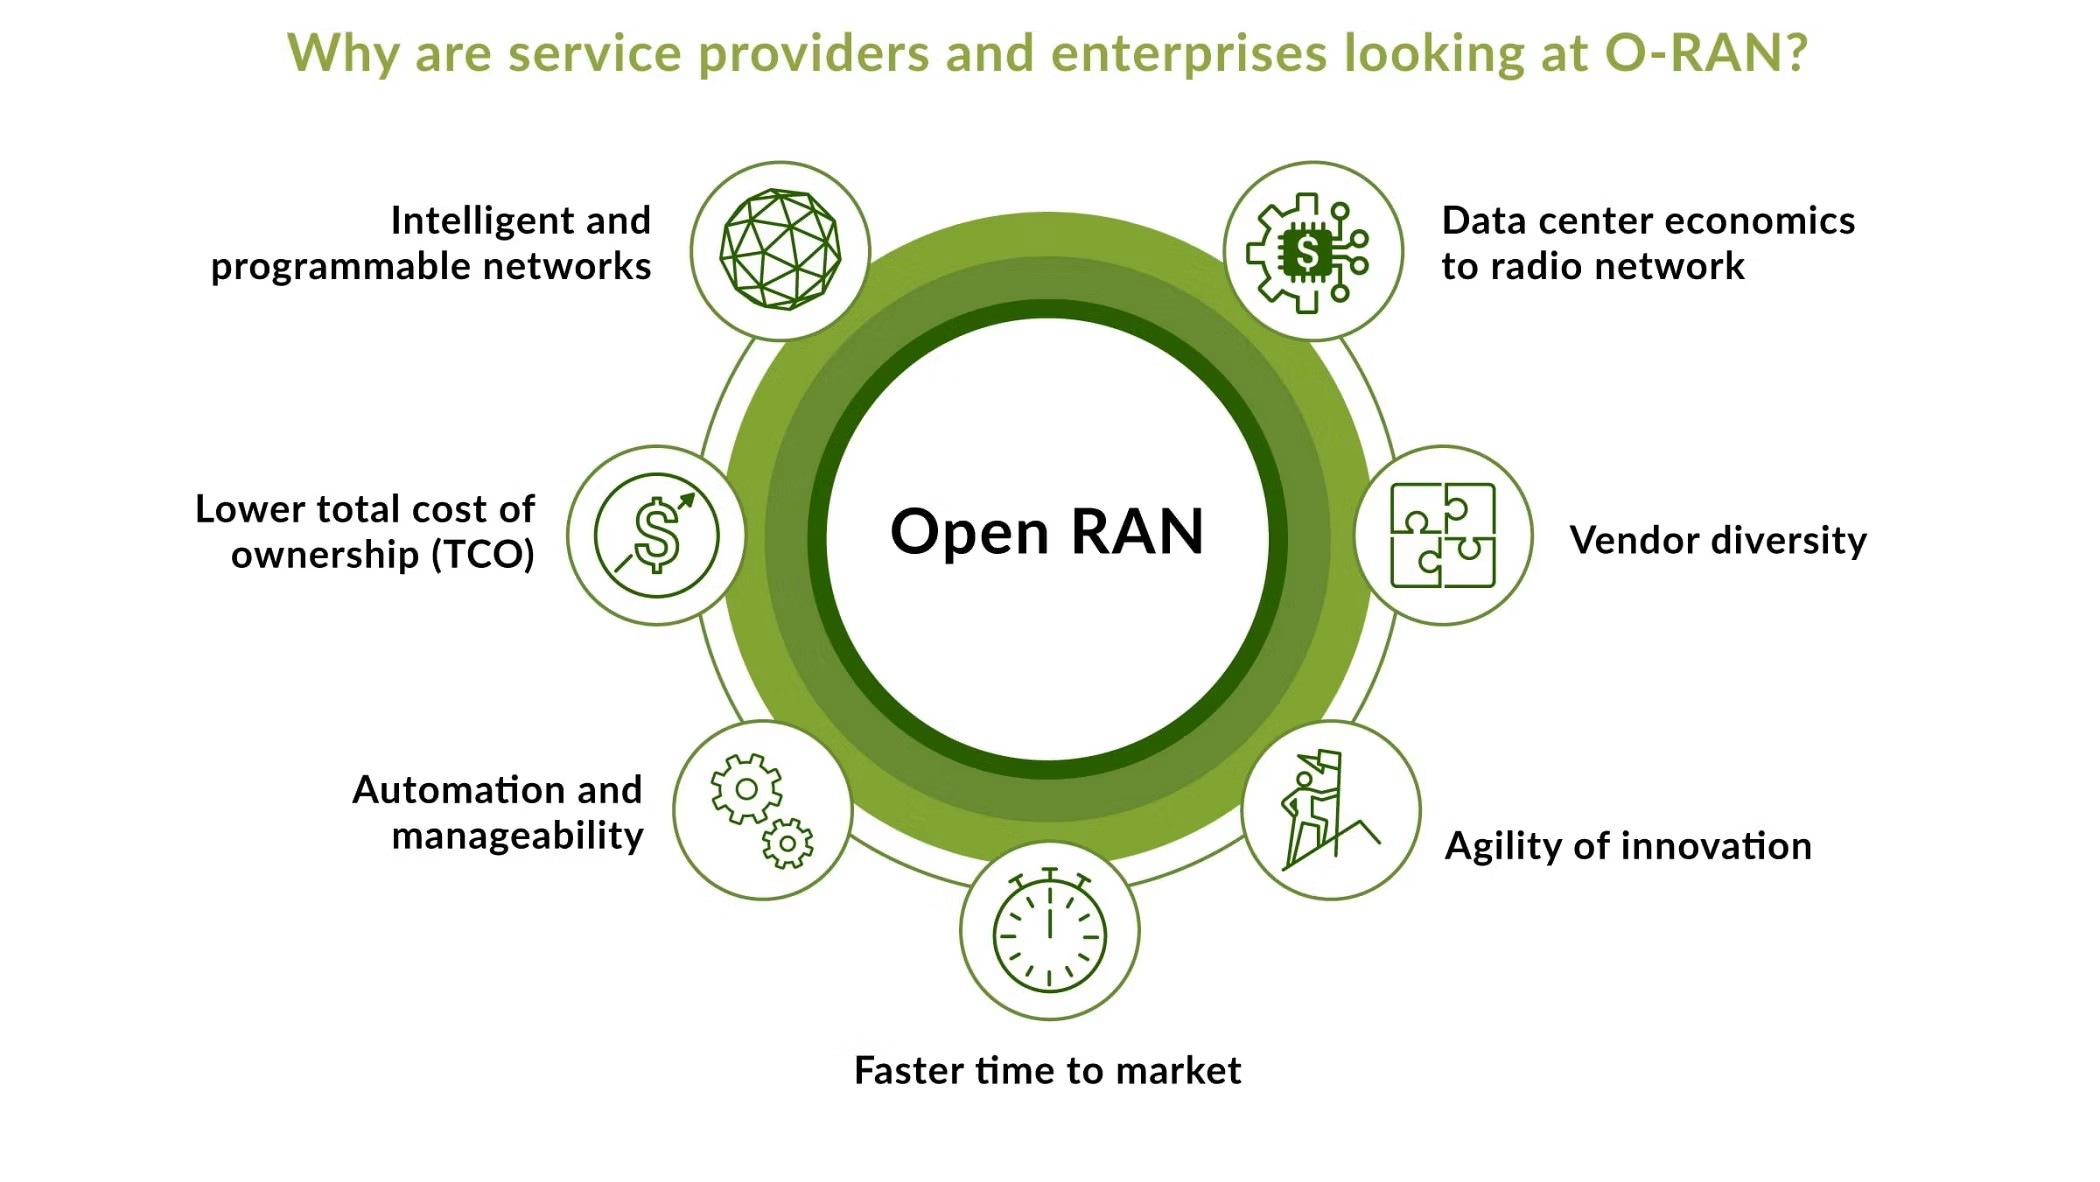
\includegraphics[width=0.6\linewidth]{figs/what-is-O-RAN.jpeg}
    \caption{O que \textit{stakeholders} procuram?\footnote{\href{https://www.juniper.net/us/en/research-topics/what-is-open-ran.html}{https://www.juniper.net/us/en/research-topics/what-is-open-ran.html}}}
\end{figure}
\end{frame}

\begin{frame}{Evolução até Open RAN}
\begin{figure}
    \centering
    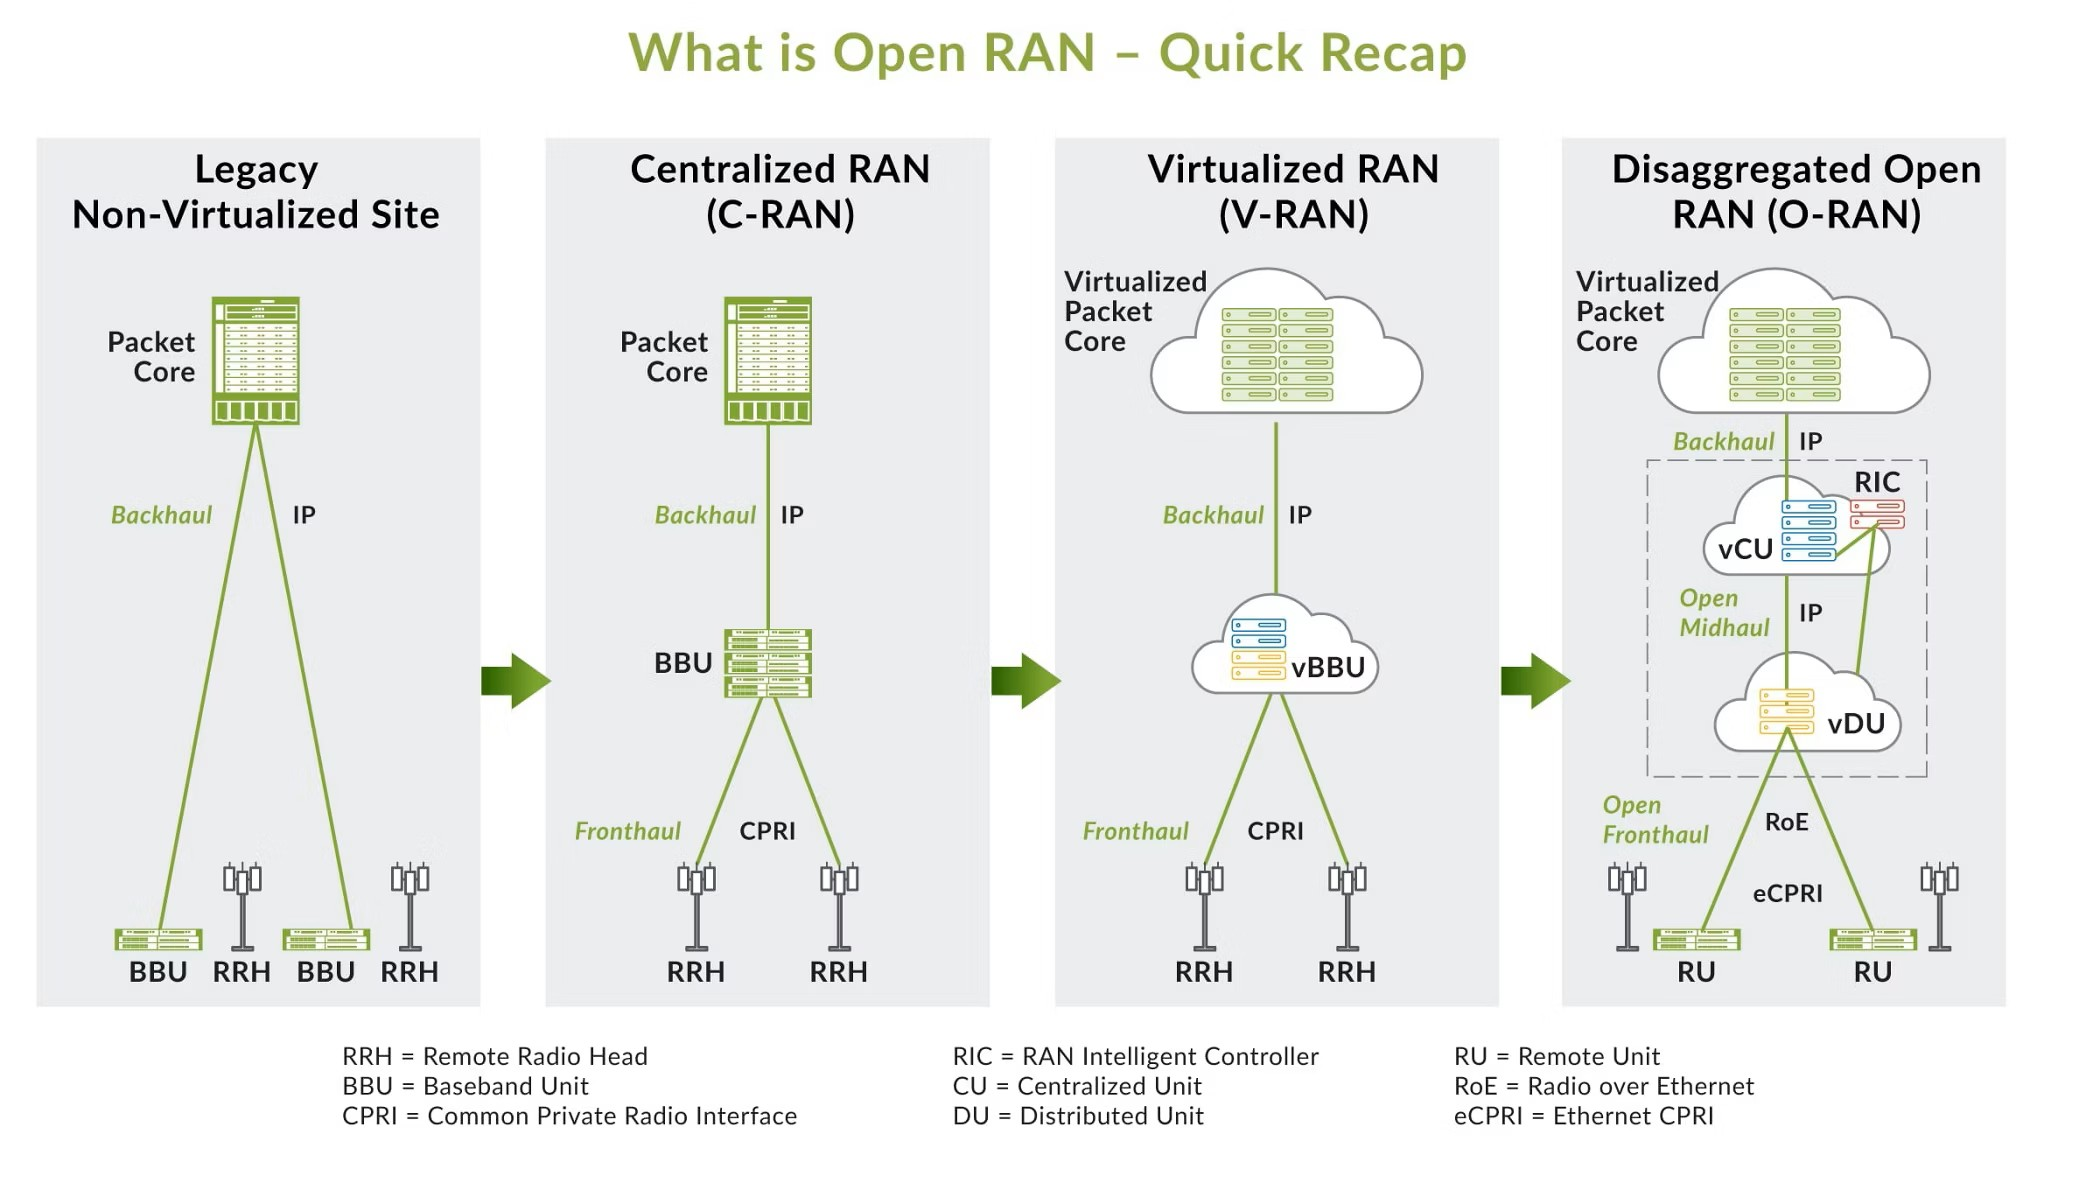
\includegraphics[width=\linewidth]{figs/what-is-O-RAN-quick-recap.jpeg}
    \caption{Recapitulando\footnote{\href{https://www.juniper.net/us/en/research-topics/what-is-open-ran.html}{https://www.juniper.net/us/en/research-topics/what-is-open-ran.html}}}
\end{figure}
\end{frame}

\begin{frame}{Arquitetura Open RAN\footcite{marques2023desagregando}}
\begin{columns}
    \begin{column}{0.5\textwidth}
    \begin{itemize}
      \item \scriptsize \textbf{SMO}: Gerenciamento e orquestração de toda a rede
    
      \item \textbf{Non-RT RIC}: Controle inteligente não em tempo real (políticas, ML/AI)
    
      \item \textbf{Near-RT RIC}: Controle quase em tempo real (10ms – 1s), otimizações dinâmicas
    
      \item \scriptsize \textbf{O-CU (Central Unit)}
            \begin{itemize}
              \item \scriptsize \textbf{O-CU-CP (Control Plane)}: sinalização e controle  
              \item \scriptsize \textbf{O-CU-UP (User Plane)}: encaminhamento de dados do usuário  
            \end{itemize}
    
      \item \scriptsize \textbf{O-DU (Distributed Unit)}: Processamento de tempo crítico (MAC, RLC, parte do PHY)  

      \item \scriptsize \textbf{O-RU (Radio Unit)}:  Processamento de rádio e funções da camada física (RF, mod/demod)  

    \end{itemize}
    \end{column}
    \begin{column}{0.5\textwidth}
        \vspace{0.5cm}
        \begin{figure}
            \centering
            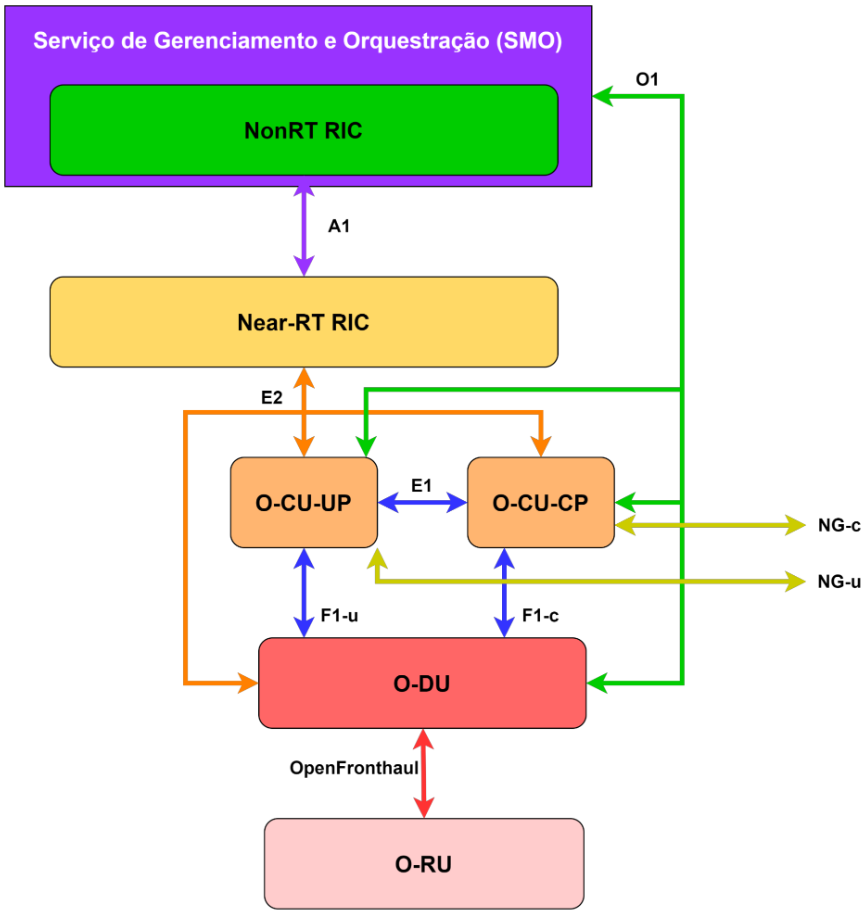
\includegraphics[width=\linewidth]{figs/arquitetura-openran.png}
            \caption{Arquitetura Open RAN\textsuperscript{4}}
        \end{figure}
    \end{column}
\end{columns}
\end{frame}

\begin{frame}{Benefícios do Open RAN}
\small
\begin{itemize}
  \item \textbf{Redução de custos CAPEX/OPEX}: uso de COTS e interfaces abertas diminui dependência de fornecedores proprietários, isso reduz investimentos iniciais e custos operacionais.
  \item \textbf{Flexibilidade e inovação}: arquitetura desagregada permite atualização modular e rápida integração de novas funcionalidades, estimulando experimentação tecnológica.
  \item \textbf{Novos players no mercado}: abertura do ecossistema cria oportunidades para startups, universidades e empresas de software, ampliando a competitividade e acelerando a evolução da rede.
  \item \textbf{Ecossistema colaborativo}: estímulo à padronização e à cooperação entre diferentes organizações, com maior diversidade de soluções e modelos de negócios.
\end{itemize}
\end{frame}

\begin{frame}{Desafios do Open RAN}
\small
\begin{itemize}
  \item \textbf{Interoperabilidade real}: necessidade de compatibilidade entre equipamentos e softwares de múltiplos fornecedores, exigindo testes extensivos e certificações.
  \item \textbf{Performance em cenários críticos}: manter níveis de latência, throughput e confiabilidade equivalentes às soluções proprietárias em ambientes de alta demanda (ex.: redes 5G industriais).
  \item \textbf{Segurança e confiabilidade}: abertura das interfaces amplia a superfície de ataque, demandando mecanismos robustos de autenticação, criptografia e monitoramento contínuo.
  \item \textbf{Resistência dos fornecedores tradicionais}: barreiras comerciais e estratégicas impostas por fabricantes estabelecidos que ainda dominam grande parte do mercado.
  \item \textbf{Complexidade de integração}: coordenação de múltiplos componentes heterogêneos aumenta os desafios de gerenciamento, operação e manutenção da rede.
\end{itemize}
\end{frame}

% Parte 4: Novos Paradigmas e Futuro
\section{Novos Paradigmas e Futuro}

\begin{frame}{Novos Paradigmas e Futuro}
\small
\begin{itemize}
  \item \textbf{Redes privadas 5G/6G}: possibilitam aplicações industriais, smart cities e setores críticos (energia, saúde, logística), com maior controle sobre segurança, QoS e confiabilidade.
  \item \textbf{IA/ML para otimização da RAN}: uso de algoritmos inteligentes para ajuste dinâmico de parâmetros, predição de tráfego, alocação eficiente de recursos e manutenção preditiva.
  \item \textbf{Orquestração com NFV, SDN e Edge}: integração de funções virtualizadas, controle centralizado e computação na borda para oferecer baixa latência e maior flexibilidade no provisionamento de serviços.
  \item \textbf{Caminho para o 6G}: evolução em direção a redes autônomas, com autoconfiguração e auto-recuperação, além de suportar casos de uso avançados como comunicação holográfica, internet tátil e integração massiva de dispositivos inteligentes.
\end{itemize}
\end{frame}


% Conclusão
\section{Conclusão}

\begin{frame}{Conclusão}
\begin{itemize}
  \item A evolução móvel abriu espaço para virtualização e desagregação
  \item A transição de redes proprietárias para COTS trouxe flexibilidade, redução de custos e novas possibilidades de inovação
  \item Open RAN quebra o paradigma dos fornecedores únicos
  \item Interfaces abertas e padronizadas promove interoperabilidade e diversidade de fornecedores, impulsionando a competição e acelerando o desenvolvimento tecnológico
  \item Futuro: redes abertas, inteligentes e orientadas a software
\end{itemize}
\end{frame}

\begin{frame}{Perguntas}
\centering
\Large Dúvidas?
\end{frame}

\begin{frame}[allowframebreaks]
\nocite{*}
\printbibliography
\end{frame}

% \begin{frame}{}
%   \centering \Large
%   \textbf{? \& | !}
% \end{frame}

\end{document}
